\documentclass[10pt,a4paper]{article}

\usepackage[margin=1.65cm]{geometry}
\usepackage{graphicx}
\usepackage{booktabs}
\usepackage{array}
\usepackage{float}
\usepackage{subcaption}
\usepackage{microtype}
\usepackage{amsmath}
\usepackage{hyperref}
\usepackage{xcolor}
\usepackage{enumitem}

\setlist{nosep,leftmargin=*}
\setlength{\parindent}{0pt}
\setlength{\parskip}{4pt}
\captionsetup{font=small}
\graphicspath{{../outputs/figures/}}

\hypersetup{
    colorlinks=true,
    linkcolor=blue,
    urlcolor=blue
}

\title{\vspace{-1.2cm}\textbf{Euro Coin Image Classification}\\
\large Machine Learning Programming Assignment}
\author{
\textbf{Name:} Yasamin Hosseinzadeh Sani \qquad
\textbf{Student ID:} 531672
}
\date{June 2026}

\begin{document}
\maketitle
\vspace{-0.7cm}

\begin{abstract}
This work develops classifiers for eight Euro coin denominations using a balanced dataset of
800 training and 160 test images. Logistic Regression, a custom convolutional neural network
(CNN), and transfer learning with MobileNetV2 were compared. Models were evaluated using both
classification accuracy and the mean absolute monetary value of misclassification. Standard
MobileNetV2 provided the best overall trade-off, achieving 78.12\% test accuracy, a mean monetary
error of 2.19 cents, and a maximum error of 40 cents. A cost-sensitive MobileNetV2 decision rule
achieved the highest accuracy, 78.75\%, but a slightly worse mean monetary error of 2.52 cents.
\end{abstract}

\section{Problem and Data Analysis}

The task is to classify images into eight classes: 1, 2, 5, 10, 20, and 50 cents, plus 1 and
2 Euro coins. Each class contains 100 training and 20 test images. All images are RGB PNG files
of size $64\times64$ pixels. The classes are therefore perfectly balanced.

The images contain substantial variation in illumination, sharpness, background, orientation,
and visible coin side. Coins may be rotated in any direction, while several denominations share
similar colour and circular geometry. As a result, raw intensity values alone are not sufficient:
a robust classifier should learn local edges, textures, relief patterns, and colour distributions,
while remaining relatively invariant to rotation, translation, and moderate illumination changes.
The brightness boxplot also shows substantial within-class spread, meaning that illumination is not
a stable class-specific cue. This is important because a classifier that over-relies on global
brightness could perform well on a limited subset of images but fail under different acquisition
conditions. These observations motivate normalisation, data augmentation, and models that preserve
spatial structure.

\begin{figure}[H]
    \centering
    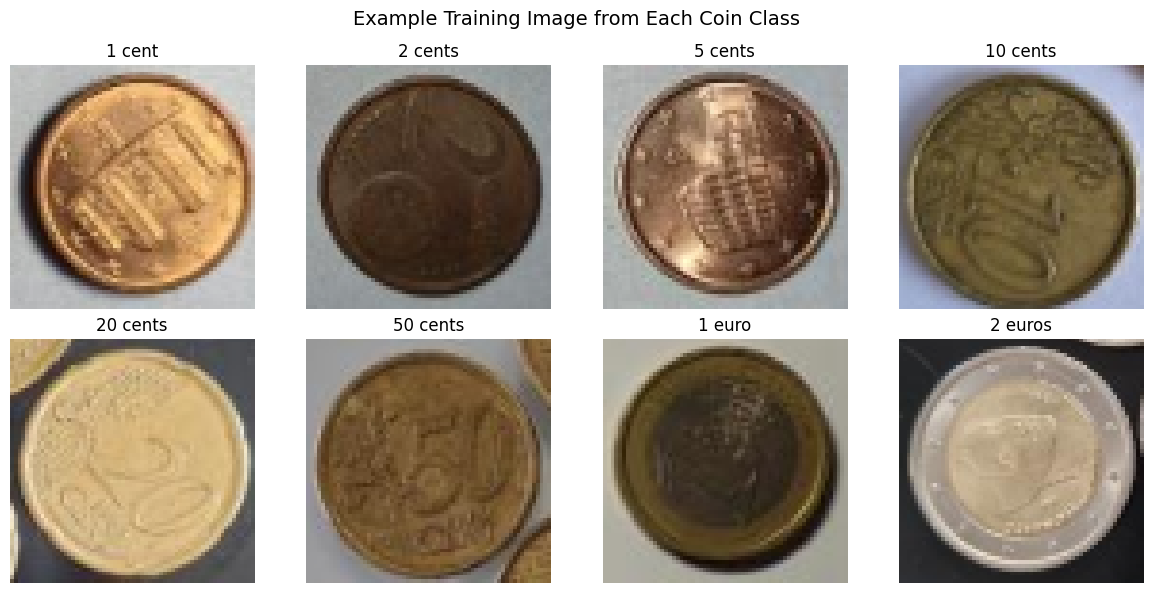
\includegraphics[width=0.82\textwidth]{notebook_figure_02_cell_011.png}
    \caption{Representative training image from each Euro coin class.}
    \label{fig:coin-examples}
\end{figure}

\begin{figure}[H]
    \centering
    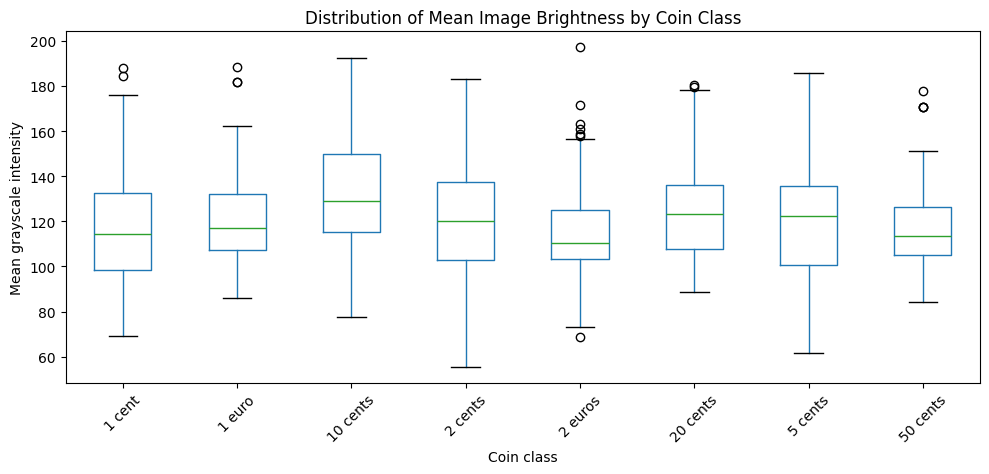
\includegraphics[width=0.7\textwidth]{notebook_figure_04_cell_018.png}
    \caption{Distribution of mean image brightness across the eight coin classes.}
    \label{fig:brightness}
\end{figure}

The 800 supplied training images were divided using a stratified 80/20 split, giving 640 training
and 160 validation images while preserving the same class proportions in both subsets. The separate
160-image test set was kept untouched during model selection and hyperparameter tuning, and was used
only once for final evaluation. This separation reduces the risk of optimistic performance estimates.

\section{Methods}

\subsection{Evaluation Criteria}

The standard classification metric was test accuracy. Precision, recall, F1-score, and confusion
matrices were also inspected in order to identify whether errors were concentrated in particular
denominations. Accuracy is appropriate because the dataset is balanced, but it treats all mistakes
as equally severe. In this application, however, confusing 1 cent with 2 cents is less costly than
confusing 20 cents with 2 Euros. Since classes represent different monetary values, the practical
cost of an error was measured as
\begin{equation}
C(y,\hat y)=|v_y-v_{\hat y}|,
\end{equation}
where $v_y$ and $v_{\hat y}$ are the true and predicted coin values in cents. The reported monetary
metric is
\begin{equation}
\mathrm{MAE}_{money}=\frac{1}{N}\sum_{i=1}^{N}|v_{y_i}-v_{\hat y_i}|.
\end{equation}

\subsection{Logistic Regression Baseline}

Each image was scaled to $[0,1]$ and flattened into $64\times64\times3=12{,}288$ features.
A pipeline containing \texttt{StandardScaler} and multinomial Logistic Regression was trained.
Standardisation places all pixel features on a comparable scale and improves numerical stability
during optimisation. This model provides an interpretable baseline, but flattening destroys the
two-dimensional neighbourhood relationships that are important for recognising rims, digits,
engravings, and bimetallic patterns. Consequently, the classifier can use colour and absolute pixel
position, but it cannot explicitly learn translation-tolerant local motifs. This limitation is
particularly relevant because the same coin may appear rotated or slightly shifted between images.

A cost-sensitive prediction rule was additionally applied to the model probabilities:
\begin{equation}
\hat y=\arg\min_j\sum_{k=1}^{8}P(y=k\mid x)\,C(k,j).
\end{equation}
This satisfies the requirement for an additional model designed to minimise the monetary value
of misclassification. Unlike the usual maximum-probability rule, this decision rule may deliberately
select a slightly less probable class when that prediction has a lower expected monetary penalty.

\subsection{Custom CNN}

The custom CNN contained three convolutional blocks, each using convolution, batch normalisation,
ReLU, and max pooling. Convolutional filters learn local visual patterns, batch normalisation
stabilises intermediate activations, and pooling progressively reduces spatial resolution while
retaining dominant features. The classifier used a fully connected layer and dropout to reduce
overfitting. Training used cross-entropy loss, Adam, weight decay, learning-rate reduction,
checkpointing, and early stopping. Augmentation included rotation, translation, scaling, and
colour jitter so that the model would not rely too strongly on a single orientation or lighting
condition. Despite this architectural advantage, the custom CNN was trained from only 640 images.
Its relatively low test accuracy suggests that learning robust visual features from scratch was
difficult under this data regime. Nevertheless, its lower monetary error indicates that many of its
mistakes occurred between nearby denominations rather than between very different coin values.

\subsection{Transfer Learning with MobileNetV2}

MobileNetV2 pretrained on ImageNet was used as the strongest classifier. Images were resized to
$160\times160$ and normalised with ImageNet statistics so that their input distribution matched
the one used during pretraining. MobileNetV2 uses depthwise separable convolutions and inverted
residual blocks, providing strong visual representations with relatively low computational cost.
The pretrained filters already encode generic edges, textures, contours, and object-part patterns,
which is advantageous when the target dataset is too small to learn all such representations from
scratch.
Training had two stages:
\begin{enumerate}
    \item freeze the feature extractor and train a new eight-class head;
    \item unfreeze the final four feature blocks and fine-tune them with a smaller learning rate.
\end{enumerate}
Moderate rotation, translation, scaling, brightness, contrast, and saturation augmentation were
applied during training. These transformations reflect the variability observed in the exploratory
analysis without introducing excessively unrealistic samples. The best checkpoint was selected by
validation loss rather than training accuracy, because validation loss also reflects prediction
confidence and is more sensitive to overfitting. The best fine-tuning checkpoint occurred at
epoch 13, with validation loss 0.5545 and validation accuracy 78.75\%.

\begin{figure}[H]
    \centering
    \begin{subfigure}{0.49\textwidth}
        \centering
        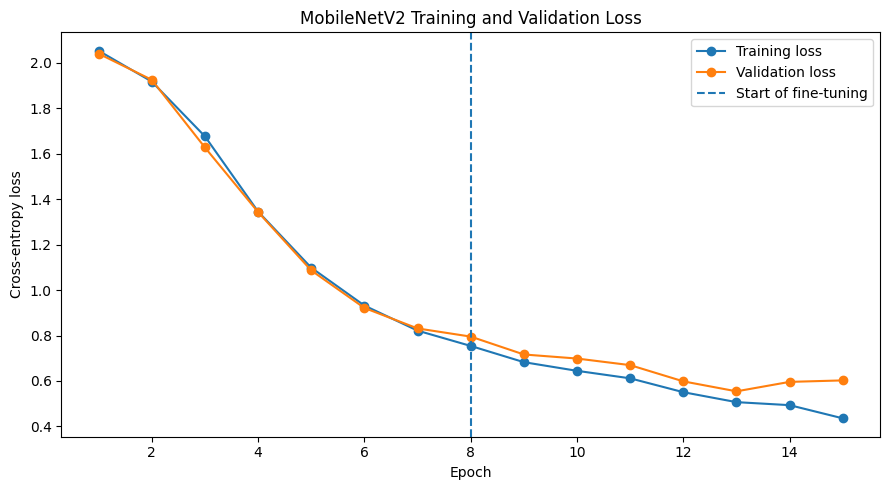
\includegraphics[width=\linewidth]{notebook_figure_14_cell_098.png}
        \caption{MobileNetV2 loss curves.}
    \end{subfigure}
    \hfill
    \begin{subfigure}{0.49\textwidth}
        \centering
        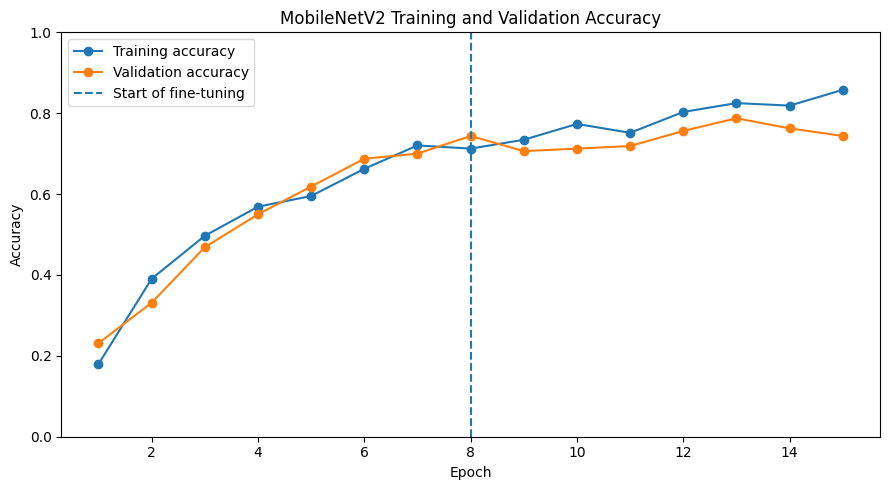
\includegraphics[width=\linewidth]{notebook_figure_15_cell_099.png}
        \caption{MobileNetV2 accuracy curves.}
    \end{subfigure}
    \caption{Training head for eight epochs, followed by fine-tuning.}
    \label{fig:mobilenet-training}
\end{figure}

The learning curves show a clear improvement during the frozen-head stage and a further gain after
fine-tuning begins. Training and validation accuracy remain relatively close for most epochs, which
suggests that the model did not severely overfit. After epoch 13, training accuracy continues to
increase while validation performance starts to fluctuate, supporting the use of validation-loss
checkpointing and early stopping.

\section{Results and Model Behaviour}

\begin{table}[H]
    \centering
    \caption{Performance on the independent 160-image test set.}
    \label{tab:results}
    \small
    \begin{tabular}{>{\raggedright\arraybackslash}p{5.4cm}ccc}
        \toprule
        \textbf{Method} & \textbf{Accuracy} &
        \textbf{Mean cost (cents)} & \textbf{Max cost (cents)}\\
        \midrule
        Logistic Regression                & 68.13\% & 8.16 & 180\\
        Cost-sensitive Logistic Regression & 68.75\% & 7.12 & 180\\
        Custom CNN                         & 61.25\% & 5.01 & 48\\
        Cost-sensitive Custom CNN          & 58.13\% & 5.67 & 95\\
        MobileNetV2                        & 78.12\% & \textbf{2.19} & \textbf{40}\\
        Cost-sensitive MobileNetV2         & \textbf{78.75\%} & 2.52 & \textbf{40}\\
        \bottomrule
    \end{tabular}
\end{table}

\begin{figure}[H]
    \centering
    \begin{subfigure}{0.49\textwidth}
        \centering
        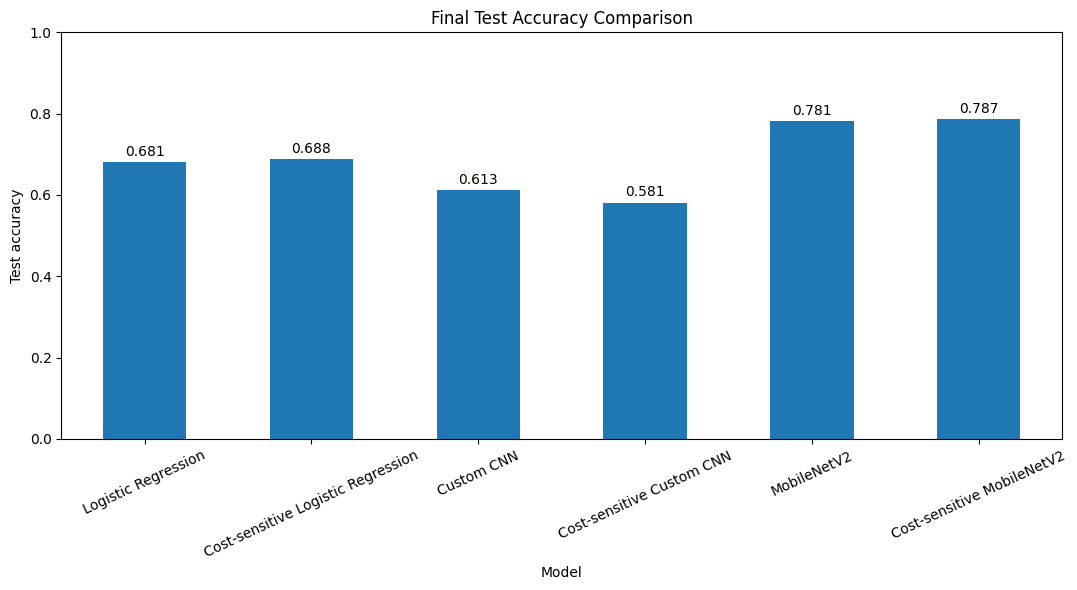
\includegraphics[width=\linewidth]{notebook_figure_17_cell_110.png}
        \caption{Accuracy comparison.}
    \end{subfigure}
    \hfill
    \begin{subfigure}{0.49\textwidth}
        \centering
        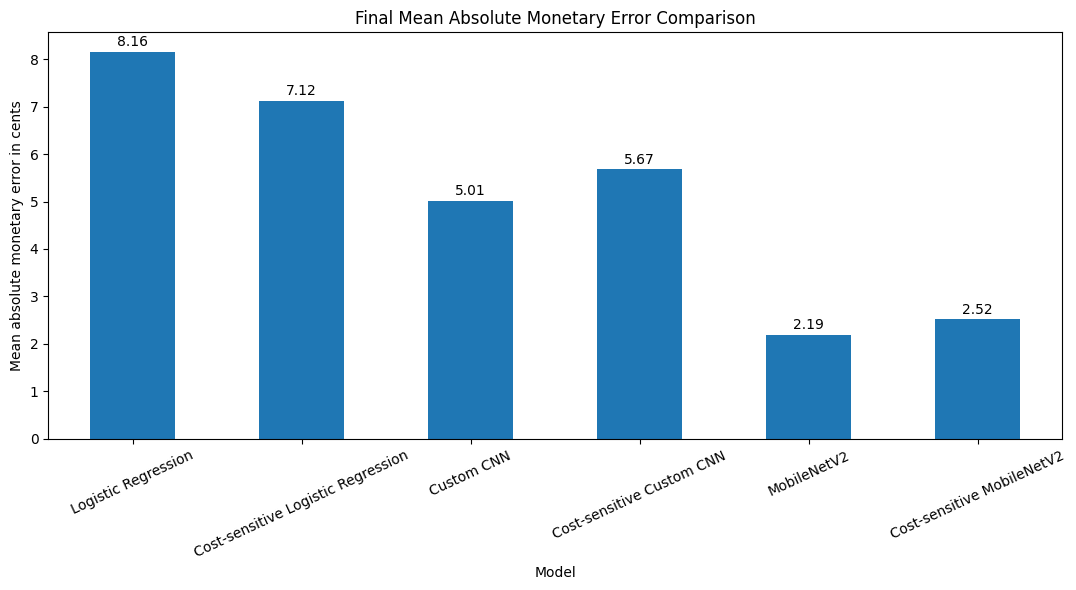
\includegraphics[width=\linewidth]{notebook_figure_18_cell_111.png}
        \caption{Mean monetary error comparison.}
    \end{subfigure}
    \caption{Final comparison of all six prediction strategies.}
    \label{fig:final-comparison}
\end{figure}

MobileNetV2 improved accuracy by 10.00 percentage points over the Logistic Regression baseline
and reduced mean monetary error by approximately 73.1\%. Its confusion matrix shows perfect
recognition of the 1 Euro and 2 Euro classes, while most remaining errors occur among visually
similar low-value cent coins. In particular, the confusions are concentrated among copper-coloured
1, 2, and 5 cent coins and among the gold-coloured 10, 20, and 50 cent coins. This pattern is
consistent with the fact that coins within each material group share similar colour and global
shape. Importantly, the largest monetary error was limited to 40 cents, showing that the remaining
mistakes were generally between economically closer denominations. Compared with Logistic
Regression, MobileNetV2 therefore improved not only the number of correct predictions but also the
severity profile of the errors. This is practically important because a classifier with similar
accuracy could still be undesirable if its few mistakes involved large value differences.

\begin{figure}[H]
    \centering
    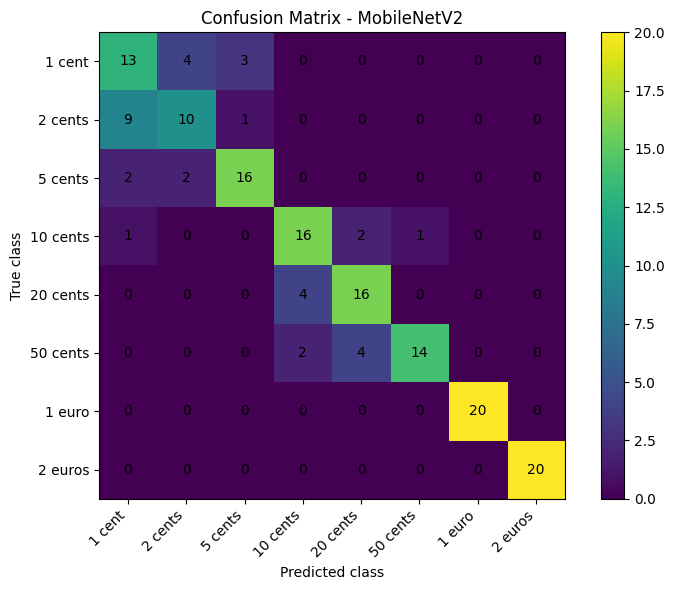
\includegraphics[width=0.54\textwidth]{notebook_figure_16_cell_103.png}
    \caption{Confusion matrix for standard MobileNetV2.}
    \label{fig:mobilenet-cm}
\end{figure}

The cost-sensitive MobileNetV2 classified one additional image correctly, but its average monetary
error increased from 2.19 to 2.52 cents. Therefore, the expected-cost decision rule did not improve
the monetary objective for this model. A plausible explanation is that the softmax probabilities
were not perfectly calibrated: if confidence values do not accurately represent true class
likelihoods, expected-cost minimisation can shift some predictions in an undesirable direction.
Standard MobileNetV2 was therefore selected as the preferred overall model because it achieved the
lowest average monetary cost while retaining nearly the highest accuracy.

The comparison between the custom CNN and Logistic Regression further illustrates the trade-off
between the two objectives. Logistic Regression achieved higher accuracy, but the custom CNN had a
lower mean and maximum monetary error. This means that the CNN made more mistakes overall, yet its
mistakes were less damaging on average. Therefore, reporting only accuracy would hide an important
aspect of model behaviour.


\section{Limitations and Possible Improvements}

The test set contains only 160 images, so small differences such as 78.12\% versus 78.75\% correspond
to only one image and should not be over-interpreted. In addition, the images are low-resolution and
may contain background information that is unrelated to the coin itself. A dedicated coin
segmentation or centre-cropping stage could reduce this source of variation. Further improvements
could include probability calibration before cost-sensitive prediction, cross-validation on the
training set, stronger but realistic rotation augmentation, and evaluation on images collected from
new cameras or environments.

\section{Reproducibility}

The experiments were implemented in Python 3.12 using NumPy, pandas, Pillow,
Matplotlib, scikit-learn, PyTorch, and TorchVision. The random seed was fixed to 42.

To reproduce the results, create and activate a virtual environment, install the
dependencies from \texttt{requirements.txt}, and run the notebook
\texttt{notebooks/euro\_coin\_classification.ipynb} from top to bottom.

The dataset must follow this directory structure:
\begin{verbatim}
data/train/{001,002,005,010,020,050,100,200}
data/test/{001,002,005,010,020,050,100,200}
\end{verbatim}

The training notebook saves model checkpoints under \texttt{outputs/models/},
figures under \texttt{outputs/figures/}, and numerical results under
\texttt{outputs/results/}.

\section{Use of AI Tools}

AI tools were used for:
\begin{itemize}
    \item explaining assignment requirements and planning the workflow;
    \item helping structure, edit, and format this report in \LaTeX.
\end{itemize}
All experiments were executed on the provided dataset, and the reported numerical results were
obtained from the submitted notebook.

\section{Conclusion}

The project analysed the dataset, trained and evaluated multiple classifiers, visualised model
behaviour, and explicitly considered the monetary cost of errors. The comparison shows that model
quality cannot be judged by accuracy alone: the custom CNN had lower accuracy than Logistic
Regression but produced less costly mistakes, whereas MobileNetV2 improved both objectives.
Transfer learning substantially outperformed both raw-pixel Logistic Regression and a CNN trained
from scratch, confirming its suitability for small image datasets. Standard MobileNetV2 was the
best overall model, combining 78.12\% accuracy with the lowest mean monetary error of 2.19 cents.
Cost-sensitive MobileNetV2 achieved the highest accuracy, 78.75\%, but did not improve monetary
cost. Further improvement could be obtained through probability calibration, larger datasets, or
coin-specific augmentation and segmentation. Overall, the results show that transfer learning is
the most effective strategy for this small image dataset, while cost-aware evaluation provides a
more complete assessment than accuracy alone.

\vfill
\begin{center}
\textit{“I affirm that this report is the result of my own work and that I did not share any part
of it with anyone else except the teacher.”}
\end{center}

\end{document}
